\section{Results (Random Operators)}
\label{sec:random-op-results}

In the previous subsections, the costs associated with LOBE are benchmarked for physically relevant models.
In this subsection, we benchmark the same costs for LOBE for randomly generated operators of form of Eq. \ref{eq:lclo}.
%\ws{@Gus, we need to describe here how the "random" protocol in OpenParticle works.}
Randomly generated operators were generated with the open-sourced package, \textit{OpenParticle} \cite{openparticle}. In OpenParticle, terms are represented by objects called \textit{ParticleOperators}. The random method takes in parameters: particle types ((anti)fermions or bosons), number of terms in the sum, then max mode and length of term. 
The random method relies on NumPy's \cite{harris2020array} random method to generate \textit{ParticleOperators} with a random configuration of terms, modes, and lengths. 

\begin{figure}
    \centering
    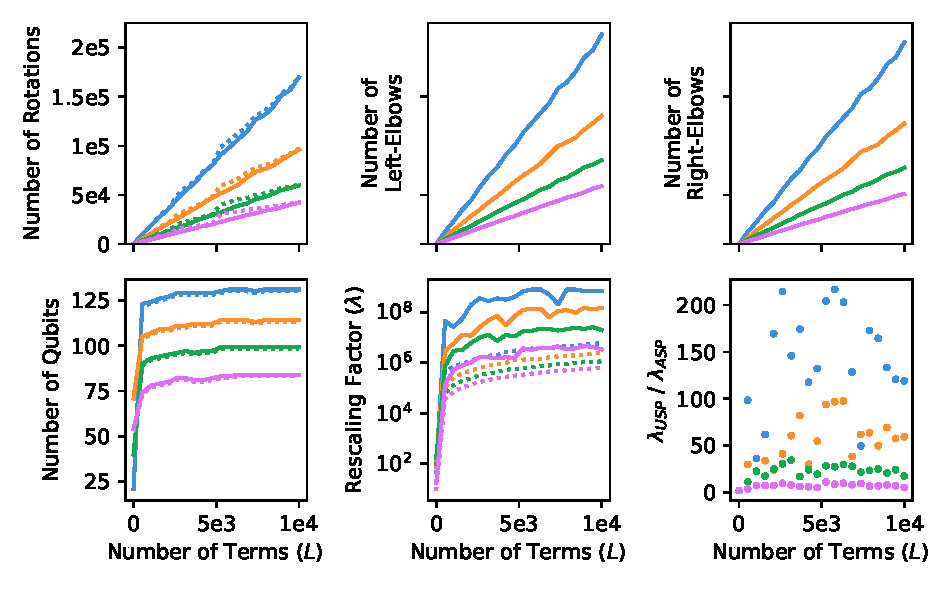
\includegraphics[width=16cm]{figures/random_hamiltonians_metrics_vs_terms.pdf}
    \caption{
        \textbf{Block-Encoding Metrics for Increasing $L$ (Random Hamiltonians).}
        The number of rotations (upper left), left-elbows (upper middle), right-elbows (upper right), number of qubits (lower left), and rescaling factors (lower middle) are plotted as a function of the number of terms in the operator ($L$).
        In the lower right subfigure, the ratio of the two rescaling factors is shown.
        The gate counts for the variant of LOBE using \textit{USP} are shown as the solid lines and those using \textit{ASP} are shown as the dotted lines.
        Metrics for different values of the bosonic occupation cutoff ($\Omega$) are represented in the different colors: $\Omega = 15$ (blue), $\Omega = 7$ (orange), $\Omega = 3$ (green), and $\Omega = 1$ (purple).
        The number of momentum modes ($I$) is set to $15$ and the maximum number of ladder operators per term is set to $5$ ($A_l + B_l + D_l \leq 5$).
        The number of rotations excludes rotations by angles that result in Clifford operations.
    }
    \label{fig:random_hamiltonians_metrics_vs_terms}
\end{figure}

\begin{figure}
    \centering
    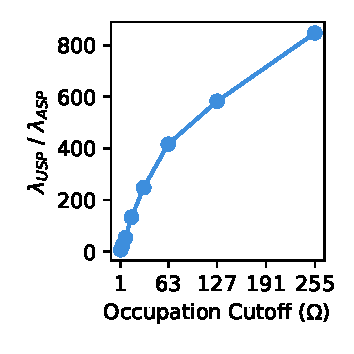
\includegraphics[width=6cm]{figures/random_hamiltonians_rescaling_factor_ratios_vs_omega.pdf}
    \caption{
        \textbf{Ratio of Rescaling Factors for Increasing $\Omega$ (Random Hamiltonians).}
        The average ratio of the two rescaling factors ($\lambda_{USP}$ and $\lambda_{ASP}$) is shown as a function of increasing bosonic occupation cutoff ($\Omega$).
        The number of momentum modes ($I$) is set to $15$ and the maximum number of ladder operators per term ($A + B$) is set to $5$.
        The ratios plotted are the average ratio over 20 unique values of $L$ linearly spaced between $1$ and $10000$.
    }
    \label{fig:random_hamiltonians_rescaling_factor_ratios_vs_omega}
\end{figure}

In Figure \ref{fig:random_hamiltonians_metrics_vs_terms}, we plot the spacetime quantum resources associated with a LOBE block-encoding for randomly generated Hamiltonians.
As is seen for the other models, the number of non-Clifford operations scales linearly with $L$ and the number of qubits scales logarithmically with $L$.
The rescaling factors for both implementations scale logarithmically with $L$.
Additionally, the ratio between the rescaling factors is seemingly independent of $L$, however does appear to increase with $\Omega$.

In Figure \ref{fig:random_hamiltonians_rescaling_factor_ratios_vs_omega}, we plot the average ratio of the rescaling factors for the two variants of LOBE as a function of $\Omega$.
The ratio increases as a function of $\Omega$, indicating that the implementation using \textit{ASP} is increasingly more favorable for models that include a large number of bosons.

